\documentclass[a4paper,14pt]{article}
\usepackage[14pt]{extsizes}




\usepackage{cmap}					% поиск в PDF
\usepackage{mathtext} 				% русские буквы в формулах
\usepackage[T2A]{fontenc}			% кодировка
\usepackage[utf8]{inputenc}			% кодировка исходного текста
\usepackage[english,russian]{babel}	% локализация и переносы
\usepackage{ulem}                   % зачеркнутый текст
\usepackage{amssymb}			% пакет математики
\usepackage{float}
\usepackage{amsmath}
\usepackage{graphicx}
\DeclareGraphicsExtensions{.png}

%%% Страница
%\usepackage{extsizes} % Возможность сделать 14-й шрифт
\usepackage[left=1cm,right=1cm,top=1cm,bottom=1cm]{geometry} % Простой способ задавать поля
\pagestyle{empty}

\begin{document}


\begin{center}
ФЕДЕРАЛЬНОЕ ГОСУДАРСТВЕННОЕ ОБРАЗОВАТЕЛЬНОЕ БЮДЖЕТНОЕ УЧРЕЖДЕНИЕ ВЫСШЕГО ОБРАЗОВАНИЯ

    \textbf{«ФИНАНСОВЫЙ УНИВЕРСИТЕТ ПРИ ПРАВИТЕЛЬСТВЕ РОССИЙСКОЙ ФЕДЕРАЦИИ»}

Факультет информационных технологий и анализа больших данных

Департамент анализа данных и машинного обучения

\textit{
	\textbf{Дисциплина: «Теория вероятностей и математическая статистика»}}

\textit{Направление подготовки: 01.03.02 «Прикладная математика и информатика»}

\textit{Профиль: «Анализ данных и принятие решений в экономике и финансах»}

\textit{Форма обучения очная, учебный 2020/2021 год, 4 семестр}

\textbf{Билет 102}

\end{center}

\begin{enumerate}


\item


Сформулируйте определение случайной выборки из конечной генеральной совокупности. Какие
виды выборок вам известны? Перечислите (с указанием формул) основные характеристики выборочной и генеральной совокупностей




Здесь очень много исчерпывающей информации о выборках из генеральной совокупности и про различные виды выборок


\item



Случайные величины $X$ и $Y$ независимы и имеют равномерное
распределение на отрезках $[0;3]$ и $[0;8]$ соответственно. Для случайной величины $Z=\frac{Y}{X}$ найдите: 
1) функцию распределения $F_Z(x)$;
2) плотность распределения $f_Z(x)$ и постройте график плотности;
3) вероятность $\P(2,\!475\leqslant Z\leqslant 4,\!811)$.




%\folder 2_53d8.png
1) Функция распределения $F_Z(x)$ имеет вид:
$
F_Z(x)=\left\{
\begin{array}{l}
0, x\leqslant 0;\\
\frac{3 x}{16}, 0\leqslant x\leqslant \frac{8}{3}\approx 2,\!667;\\
1 - \frac{4}{3 x}, x\geqslant\frac{8}{3};
\end{array}.
\right.
$
2) Плотность распределения $f_Z(x)$ имеет вид:
$
f_Z(x)=\left\{
\begin{array}{l}
0, x<0;\\
\frac{3}{16}, 0\leqslant x\leqslant \frac{8}{3}\approx 2,\!667;\\
\frac{4}{3 x^{2}}, x\geqslant\frac{8}{3};
\end{array}.
\right.
$


\begin{figure}[H]
    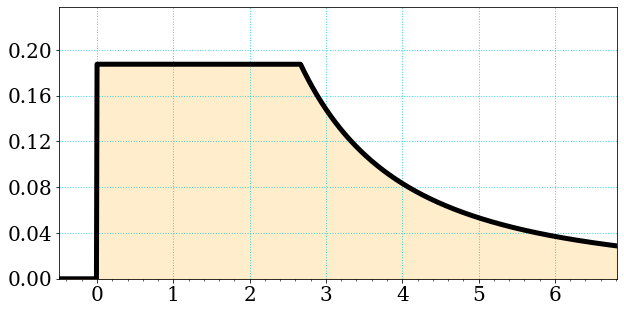
\includegraphics[width=0.9\textwidth]{2_53d8}
\end{figure}


3) вероятность равна:
$
\P(2,\!475\leqslant Z\leqslant 4,\!811)=
0,\!25884.
$


\item

    
	Случайная величина Y принимает только значения из множества $\{1, 10\}$, при этом $P(Y=1) = 0.7$.
	Распределение случайной величины X определено следующим образом:
	\begin{equation*}
		X | Y =
		\begin{cases}
			$5$ * y, с вероятностью $ 0.11$ \\
			$8$ * y, с вероятностью $ 1 - 0.11$
		\end{cases}
	\end{equation*}

	Юный аналитик Дарья нашла матожидание и дисперсию $X$.

	Помогите Дарье найти матожидание и дисперсию величины $X$
	


	

	Первым этапом надо найти характеристики случайной величины $Y$

	$E(Y) = 1 * 0.7 + 10 * (1 - 0.7)$

	$Var(Y) = E(Y^2) - [E(Y)]^2 = 1^2 * 0.7 + 10^2 * (1 - 0.7) - [E(Y)]^2$


	Перейдем к рассмотрению характеристик условной случайно величины X

	$E(X) = E(E(X|Y)) = E[E(5 * Y) * 0.11 + E(8 * Y) * (1 - 0.11)] = E(Y) * (5 * 0.11 + 8 * (1 - 0.11)) = 28.379$

	$E(Var(X|Y)) = E[b * Var(c3 * Y) + (1 - b) * Var(c4 * Y)] = Var(Y) * (c3^2 * b + c4^2 * (1- b)) $

	$Var(E(X|Y)) = E(X^2|Y) - [E(X)]^2 = [E(Y)]^2 * (b * c3^2 + (1-b)*c4^2) - E(X)]^2$

	$Var(X) = E(Var(X|Y)) + Var(E(X|Y)) = 1027.72936$
	

\item


(10) В группе $\Omega$ учатся студенты:$\omega _{1}...\omega _{25}$ . Пусть $X$ и $Y$ – 100-балльные экзаменационные оценки по
математическому анализу и теории вероятностей. Оценки $\omega _{i}$ студента обозначаются: $x _{i} = X(\omega _{i})$ и $y _{i} = Y(\omega _{i})$, $i = 1...25$. Все оценки известны
$x _{0} = 33, y _{0} = 72$, $x _{1} = 94, y _{1} = 94$, $x _{2} = 91, y _{2} = 52$, $x _{3} = 47, y _{3} = 59$, $x _{4} = 53, y _{4} = 45$, $x _{5} = 96, y _{5} = 54$, $x _{6} = 60, y _{6} = 99$, $x _{7} = 70, y _{7} = 44$, $x _{8} = 50, y _{8} = 81$, $x _{9} = 57, y _{9} = 40$, $x _{10} = 99, y _{10} = 61$, $x _{11} = 94, y _{11} = 43$, $x _{12} = 85, y _{12} = 96$, $x _{13} = 30, y _{13} = 91$, $x _{14} = 57, y _{14} = 37$, $x _{15} = 42, y _{15} = 35$, $x _{16} = 84, y _{16} = 75$, $x _{17} = 96, y _{17} = 97$, $x _{18} = 69, y _{18} = 92$, $x _{19} = 91, y _{19} = 93$, $x _{20} = 45, y _{20} = 30$, $x _{21} = 35, y _{21} = 94$, $x _{22} = 83, y _{22} = 53$, $x _{23} = 53, y _{23} = 60$, $x _{24} = 36, y _{24} = 69$
Требуется
найти следующие условные эмпирические характеристики: 1) ковариацию $X$ и $Y$ при условии, что одновременно $X \geqslant 50$
 и $Y \geqslant 50$; 2) коэффициент корреляции $X$ и $Y$ при том же условии.




1) Ковариация = $-350.8333$
2) Коэффициент корреляции = $-1.2925$


\item


(10) Эмпирическое распределение признаков $X$ и $Y$ на генеральной совокупности $\Omega$ задано таблицей частот  
 
\begin{tabular}{ | c | c | c | c | }
\hline
 & $Y = 2$ & $Y = 4$ & $Y = 5$  \\ \hline
$X = 200$ & $25$ & $26$ & $10$\\ \hline
$X = 300$ & $10$ & $10$ & $19$\\
\hline
\end{tabular}

Из $\Omega$ случайным образом без возвращения извлекаются $12$ элементов. 
Пусть $\bar X$ и $\bar Y$ – средние значения признаков на выбранных элементах. 
Требуется найти: 1) математическое ожидание $\mathbb{E}(\bar Y)$; 2) стандартное отклонение $\sigma(\bar X)$ ; 
3) ковариацию $Cov(\bar X, \bar Y)$




1) математическое ожидание $\mathbb{E}(\bar Y)$: $3.59$ 
2) стандартное отклонение $\sigma(\bar X)$: $228.8693$
3) ковариацию $Cov(\bar X, \bar Y)$: $1.3324$


\item

    
	Известно, что доля возвратов по кредитам в банке имеет распределение $F(x) = x^{\beta}, 0 \le x \le 1$. Наблюдения показали, что в среднем она составила $71.0$\%. Методом моментов оцените параметр $\beta$ и вероятность того, что она опуститься ниже $62.0$\%.
	


	

	$f(x) = F'(x) = \beta \cdot x^{\beta - 1}$

	$\mu_{1} = E(X) = \int_{-\inf}^{\inf}x \cdot f(x) = \int_{-\inf}^{\inf} \beta \cdot x^{\beta} = \beta \cdot \frac{x^{\beta + 1}}{\beta + 1}\bigg|_0^1 = \frac{\beta}{\beta + 1}$

	$\beta = (\beta + 1) \cdot 71.0$

	$\beta = \frac{71.0}{1 - 71.0}$

	$ P(x \le 62.0) = F(62.0) = 62.0^{2.45} $

    Ответ: $2.45, 0.31$
	

\end{enumerate}

\begin{figure}[H]
	Подготовил
	\hfill
	
\includegraphics[width=2cm]{Prepared}
	П.Е. Рябов
\end{figure}


\begin{figure}[H]
	Утверждаю:\\
	Первый заместитель\\
	руководителя департамента\\
	Дата 01.06.2021
	\hfill
	
\includegraphics[width=2cm]{Approved}
	Феклин В.Г.
\end{figure}

\end{document}

